\documentclass[12pt, dvipsnames, svgnames, x11names,]{article}

\usepackage{xcolor}
% URLs and hyperlinks ---------------------------------------
\usepackage{hyperref}
\hypersetup{
	colorlinks=true,
	linkcolor=NavyBlue,
	filecolor=magenta,      
	urlcolor=blue,
}
\usepackage{xurl}
%---------------------------------------------------
\usepackage[inline]{enumitem}
\usepackage{graphicx}
\usepackage{multirow}
\usepackage{float}
\renewcommand{\arraystretch}{1.40}

% adjust a verrrrry big table -------------------------------
\usepackage{adjustbox}
% -----------------------------------------------------------

\usepackage{array}
% center the p columns and m --------------------------------------------------------------
\newcolumntype{P}[1]{>{\centering\arraybackslash}p{#1}}
\newcolumntype{M}[1]{>{\centering\arraybackslash}m{#1}}
% -------------------------------------------------------------------------------------------------------------

% price
\usepackage{marvosym}
% ----------

\usepackage{xepersian}
\settextfont{Arial}
\setdigitfont{Arial}

\begin{document}
	\begin{titlepage}
		\centering
		\vspace{1cm}
		{\Huge {\textbf{\lr{BM25 Ranking}}}\par}
		\vspace{15mm}
		\vspace{16mm}
		
\includegraphics[width=13cm]{images/00.png} \par
		\vfill \par	\vfill
		\vspace{16mm}
		{\normalsize	سیدمحمدحسین هاشمی  4022363143 \par}
		\vspace{1cm}
		{\large فروردین ۱۴۰3\par}
	\end{titlepage}
	\tableofcontents
	\newpage
	
		
	
	\section{کتابخانه‌های مورد نیاز}
	
		\begin{center}
			{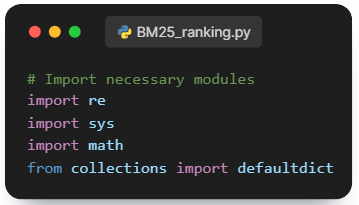
\includegraphics[width=6cm]{images/01.png}}
		\end{center}
	
		{\normalsize کتابخانه‌های مورد نیاز که در پروژه لود شده‌اند.}
	
	
	
	\section{کلاس \lr{Inverted Index}}
	
		\begin{center}
			{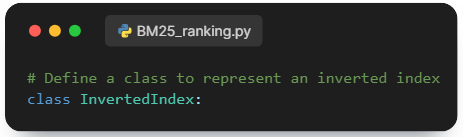
\includegraphics[width=7cm]{images/02.png}}
		\end{center}
	
		{\normalsize تمام کدهای مربوطه در این کلاس نوشته می‌شود}
	
				
	
	\section{متد \lr{--init--}}
		\begin{center}
			{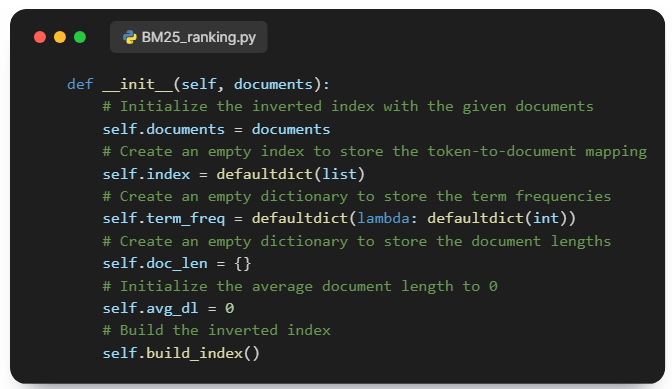
\includegraphics[width=9cm]{images/03.png}} \par
		\end{center}
		
		{\normalsize  بدر اینجا داکیومنت‌ها به عنوان ورودی دریافت شده و پس از تعریف متغیرهای مورد نیاز با فراخوانی \lr{build\_index}، \lr{Inverted Index} ایجاد می‌شود.}
	
	
	\section{متد \lr{build\_index}}
	
		\begin{center}
			{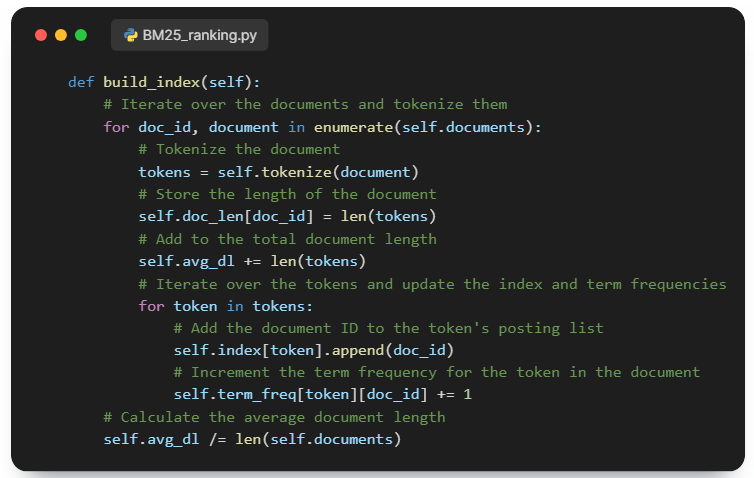
\includegraphics[width=10cm]{images/04.png}} \par
		\end{center}
		
		{\normalsize
			در این تابع \lr{Inverted Index} ساخته‌می‌شود وعلاوه بر آن طول هر داکیومنت به همراه میانگین طول داکیومنت‌ها محاسبه می‌شود.
		} \par

	
	
	\section{متد \lr{tokenize}}
		
		\begin{center}
			{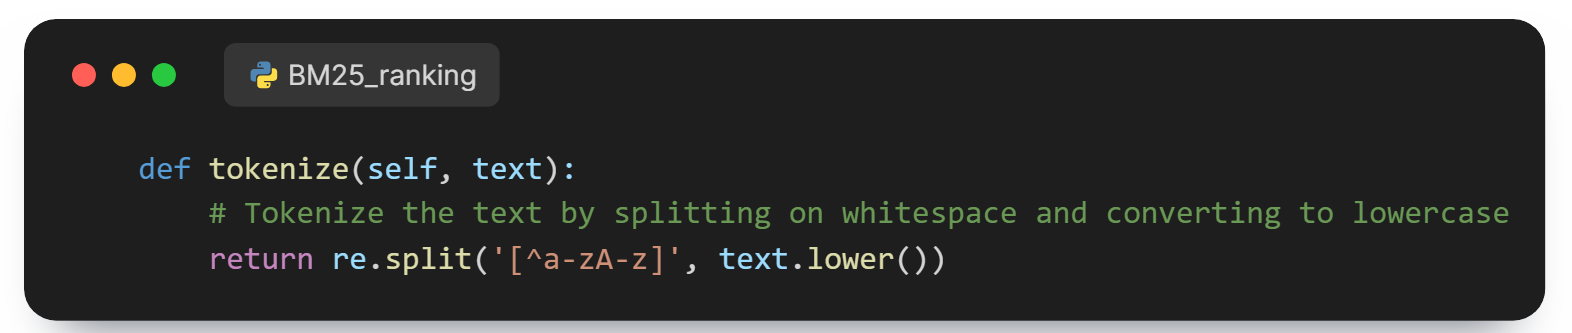
\includegraphics[width=10cm]{images/05.png}} \par
		\end{center}
		
		{\normalsize 
			در این متد از کلمات از متن استخراج می‌شوند.
		}
		
		
	
	\section{متد \lr{bm25\_score}}
	
		\begin{center}
			{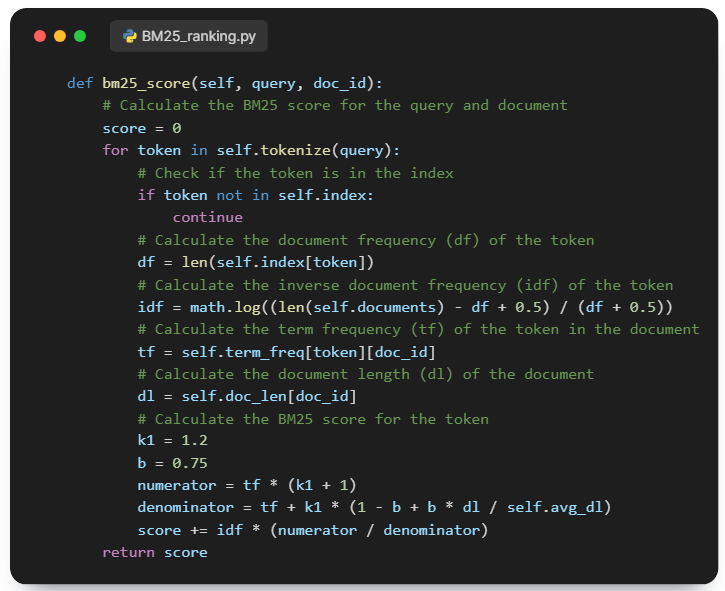
\includegraphics[width=10cm]{images/06.png}} \par
		\end{center}
		
		{\normalsize 
			در اینجا داکیومنت‌ها بر اساس فرمول \lr{BR25} امتیازدهی می‌شوند که فرمول آن به‌شرح زیر است: 
		}
		
		$$
		 score(d) = \sum_{t \in q} \left( 
		 \frac{f_{t,d} \cdot (k_1 + 1)}
		 {k_1 \cdot \left( (1-b) + b \cdot \frac{|d|}{avgdl} \right) + f_{t,d}}
		 \right) \cdot \log\left( 
		 \frac{N - n_t + 0.5}{n_t + 0.5}
		 \right) \cdot 
		 \frac{(k_2 + 1) \cdot f_{t,q}}
		 {k_2 + f_{t,q}}
		 \label{eq:bm25_inverse_index}
		$$

	
	\section{متد \lr{search}}
	
		\begin{center}
			{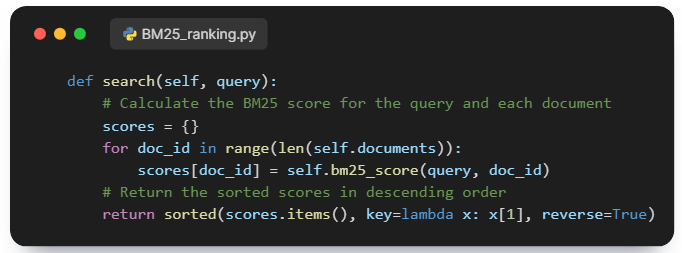
\includegraphics[width=10cm]{images/07.png}} \par
		\end{center}
		
		{\normalsize 
			در این متد کلمات از رشته ورودی استخراج شده و پس از آن با استفاده از متد \lr{bm25\_score} دسته بندی می‌شوند و براساس امتیاز مرتب شده و برگشت‌داده می‌شود.
		}
		
		
	\section{استفاده}
	
		\begin{center}
			{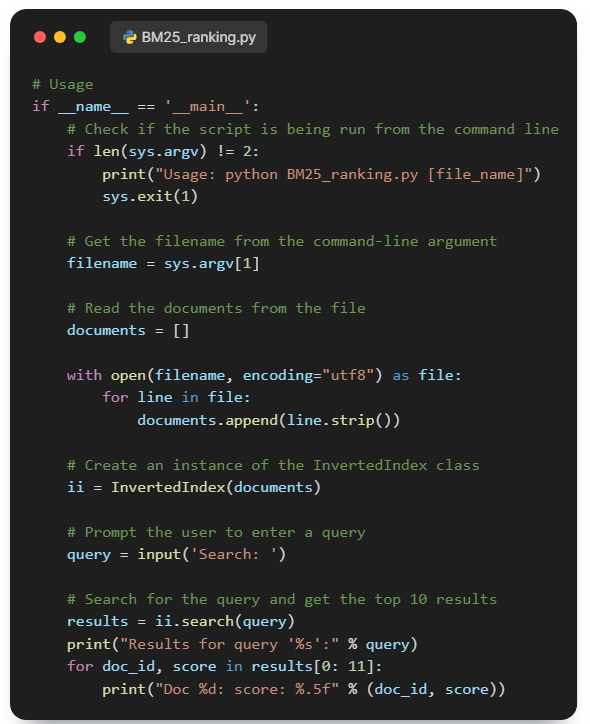
\includegraphics[width=10cm]{images/08.png}} \par
		\end{center}
		
		{\normalsize 
			برای استفاده از کلاس گفته شده این کد نوشته شده که بعد از فراخوانی کلاس ایجاد شده و پس از خواندن داکیومنت‌ها و ایجاد \lr{Inverted Index} در آن با استفاده از رنکینگ \lr{BM25} جست‌و‌جو انجام می‌شود و 10 نتیجه اول به همراه امتیاز خروجی داده می‌شود.
		}		
		
		{\normalsize برای مثال برای ورودی مانند تصویر زیر:}
		
		\begin{center}
			{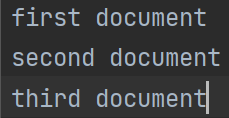
\includegraphics[width=6cm]{images/09.png}} \par
		\end{center}
		
		{\normalsize خروجی مانند تصویر زیر تولید می‌شود.}
		
		\begin{center}
			{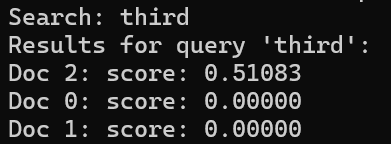
\includegraphics[width=6cm]{images/10.png}} \par
		\end{center}
	
\end{document}